
\documentclass[aspectratio=169]{beamer}
\usetheme{Madrid}
 
\usepackage{graphicx}
\usepackage[spanish]{babel}
\usepackage[utf8]{inputenc}

%\setbeamertemplate{footline}[frame number]

\begin{document}

\title{
	\textbf{Introduction to neural networks}} 
\subtitle{Machine learning recall} 
\author[J.I. Vasquez]{\textbf{Juan Irving Vásquez}}
\date{\today}
\institute[jivg.org]{ Instituto Politécnico Nacional \\Centro de Innovación y Desarrollo Tecnológico en Cómputo\\ jivg.org}
\titlegraphic{
\includegraphics[height=1.2cm]{ipn-cidetec.png}\hspace{0.1cm}
\includegraphics[height=1.2cm]{escudoESCOM}}
\frame{\titlepage} 

\begin{frame}
\frametitle{Overview} 
\tableofcontents
\end{frame}


\section{Introduction to machine learning}

{ \usebackgroundtemplate{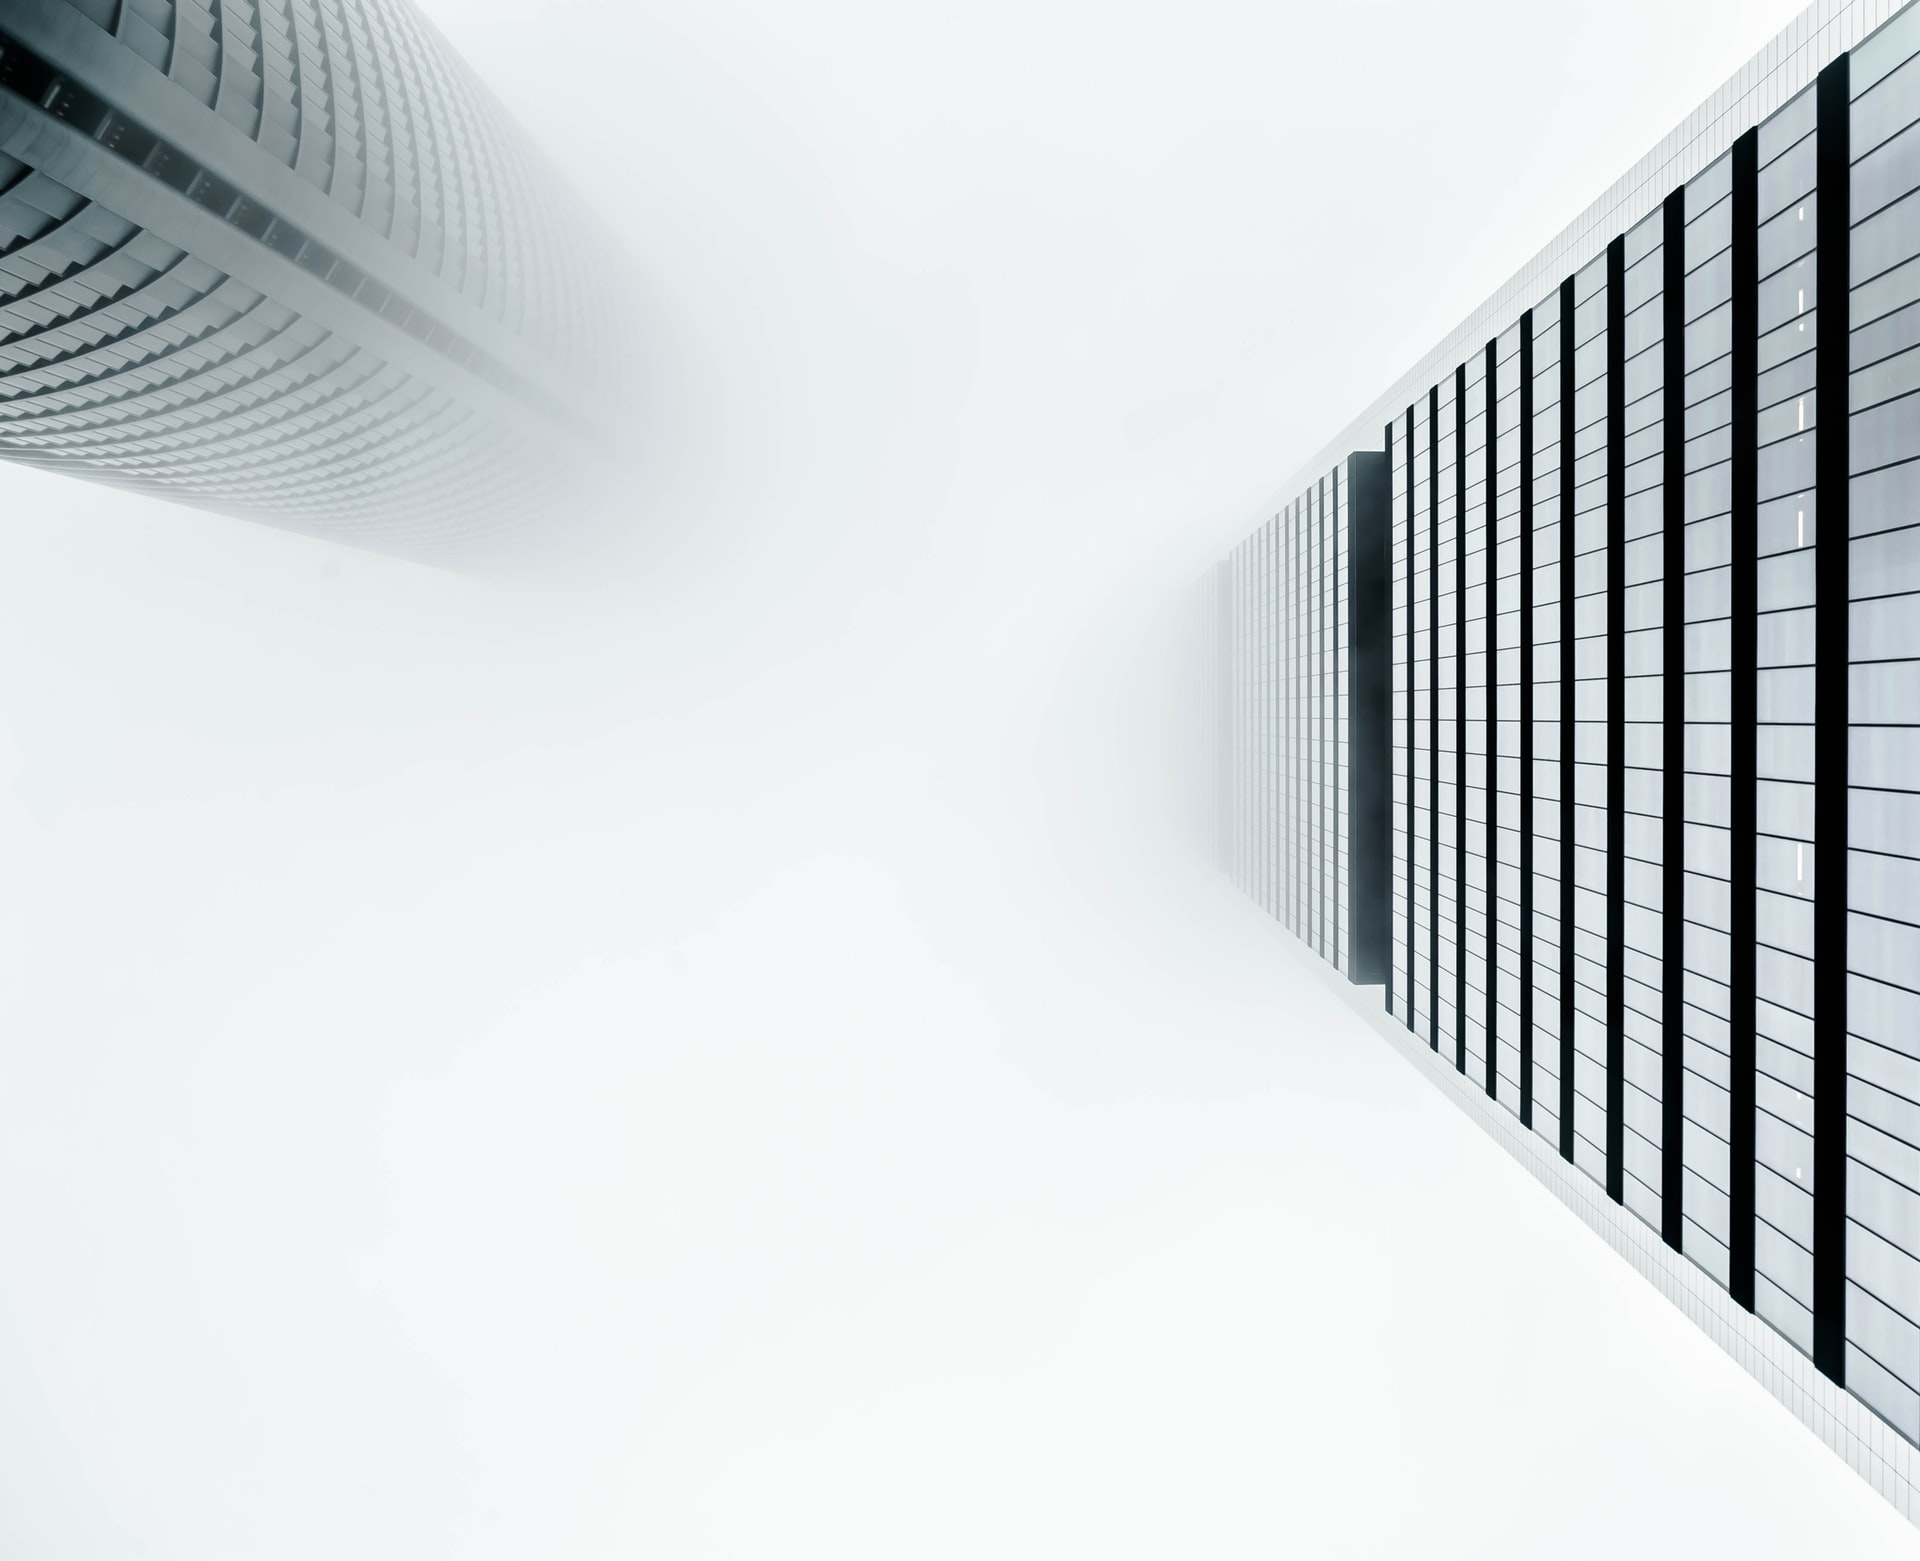
\includegraphics[width=1.0\paperwidth]{joel-filipe-VuwAfoHpxgs-unsplash}}%
\begin{frame}
	\frametitle{Introduction}
\begin{block}{Machine Learning}
	A field of study that gives computers the ability to learn without being explicitly programmed \footnote{Arthur Samuel, 1959}
\end{block}
\end{frame}
}


\begin{frame}
	\frametitle{Introduction}
\begin{block}{Learning}
An agent is learning if it improves its performance on future tasks after making observations about the world. \footnote{Russell and Norvig}    
\end{block}
\end{frame}


\begin{frame}{Machine Learning in Artificial Intelligence \footnote{\tiny Goodfellow, I., Bengio, Y., and Courville, A. (2016). Deep learning. MIT press.}}
\begin{figure}
    \centering
    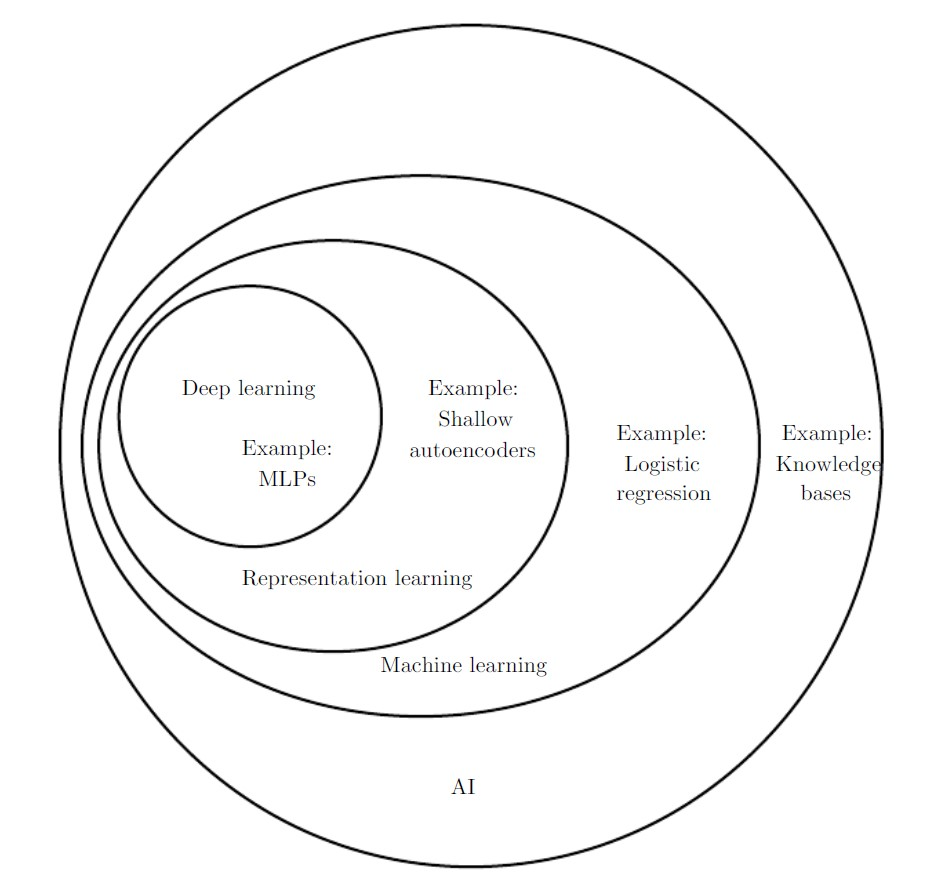
\includegraphics[width=0.45\textwidth]{deeplearning.jpg}
    %\caption{Caption}
    \label{fig:my_label}
\end{figure}
\end{frame}





\section{Machine learning tasks}

% \begin{frame}
% \frametitle{Machine Learning}
% \framesubtitle{Tasks}
% \begin{itemize}
%     \item \textbf{Regression.} Finds a function that relates the input to a continuous codomain.
% 	\pause
% 	\item \textbf{Classification.} Assigns a label to a given input. The set of classes is predefined.
% 	\pause
% 	\item \textbf{Clustering.} Automatically groups the inputs according to their features. The number of groups may be unknown.
% 	\pause
% 	\item \textbf{Dimensionality reduction.} Describes an entity with less features.
% 	\pause
% 	\item \textbf{Generative modeling.} To create new instances from a distribution.
% \end{itemize}
% \end{frame}


% Include
% hypotesis space
% Consistency of the hypothesis
\begin{frame}
\frametitle{Machine Learning}
\framesubtitle{Tasks}
\begin{itemize}
    \item \textbf{Regression.} Finds a function that relates the input to a continuous codomain.
\end{itemize}
\begin{figure}
    \centering
    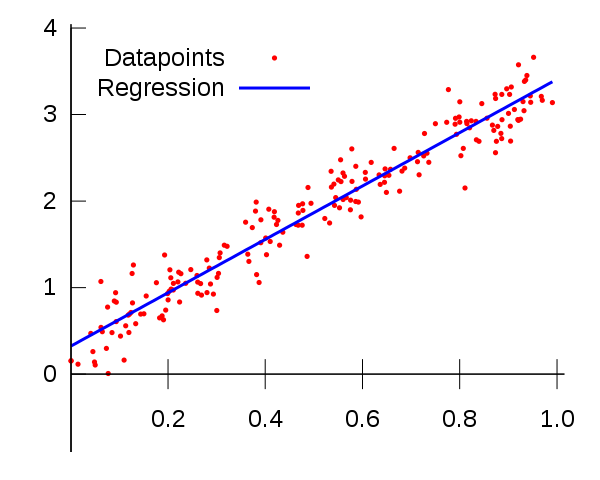
\includegraphics[height=0.7\textheight]{1_iuqVEjdtEMY8oIu3cGwC1g.png}
    %\caption{Caption}
    %\label{fig:my_label}
\end{figure}
\end{frame}
    
% Insert generalization
\begin{frame}
\frametitle{Machine Learning}
\framesubtitle{Tasks}
\begin{itemize}
	\item \textbf{Classification.} Assigns a label to a given input. The set of classes is predefined.
\end{itemize}
\begin{figure}
    \centering
    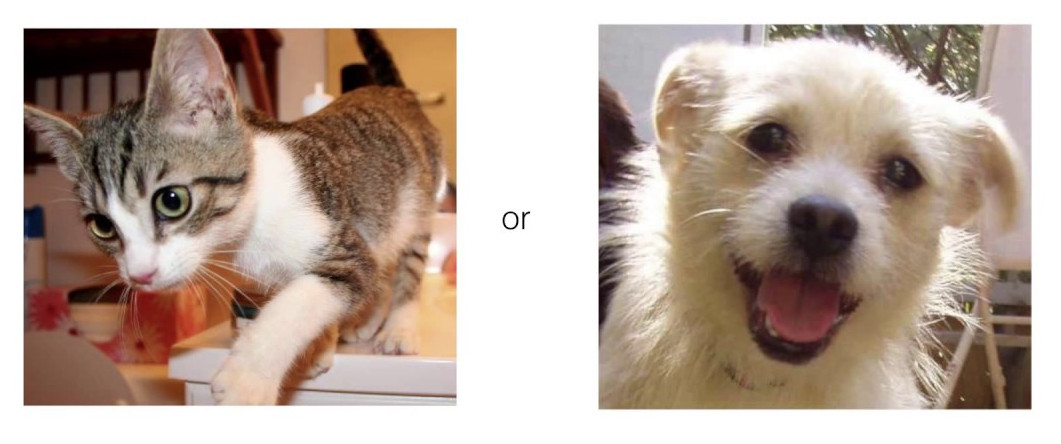
\includegraphics[height=0.6\textheight]{maxresdefault.jpg}
    %\caption{Caption}
    %\label{fig:my_label}
\end{figure}
\end{frame}

\begin{frame}
\frametitle{Machine Learning}
\framesubtitle{Tasks}
\begin{itemize}
	\item \textbf{Clustering.} Automatically groups the inputs according to their features. The number of groups may be unknown.
\end{itemize}
\begin{figure}
    \centering
    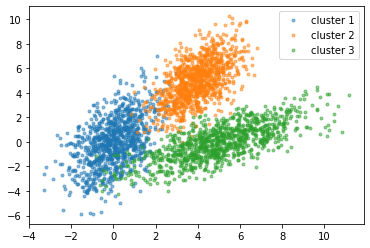
\includegraphics[height=0.6\textheight]{data_after_clustering.png}
    %\caption{Caption}
    %\label{fig:my_label}
\end{figure}
\end{frame}


\begin{frame}
\frametitle{Machine Learning}
\framesubtitle{Tasks}
\begin{itemize}
	\item \textbf{Dimensionality reduction.} Describes an entity with less features.
\end{itemize}
\begin{figure}
    \centering
    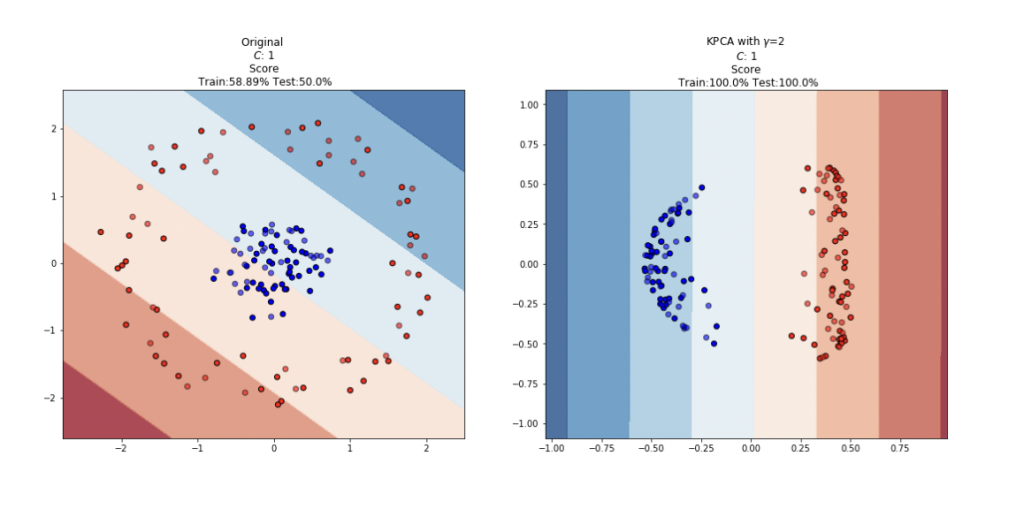
\includegraphics[height=0.7\textheight]{Dimensionality-Reduction-for-Machine-Learning_2.png}
    %\caption{Caption}
    %\label{fig:my_label}
\end{figure}
\end{frame}

\begin{frame}
\frametitle{Machine Learning}
\framesubtitle{Tasks}
\begin{itemize}
	\item \textbf{Generative modeling.} To create new instances from a distribution.
\end{itemize}
\begin{figure}
    \centering
    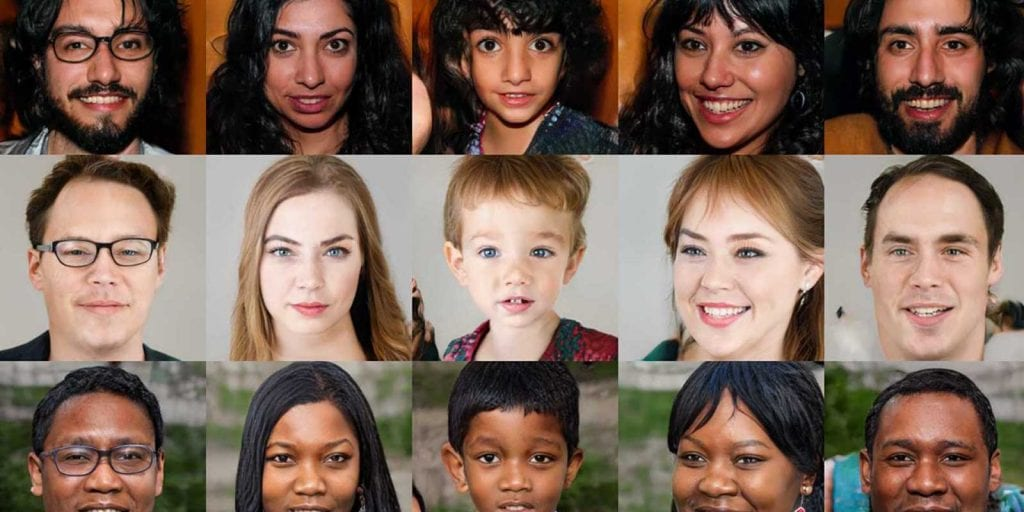
\includegraphics[height=0.6\textheight]{ai_research_gan_1600px_web-1024x512.jpg}
    %\caption{Caption}
    %\label{fig:my_label}
\end{figure}
\end{frame}




%\section{Classification}

% \frame{
% 	\frametitle{Classification}
% 	\begin{itemize}
% 		\item "The computer program is asked to specify which of k categories some input belongs to". [Goodfellow]
% 		\begin{equation}
% 		f:\mathbb{R}^n \rightarrow \{1, \dots, k\}
% 		\end{equation}
% 		\begin{figure}
% 			\centering
% 			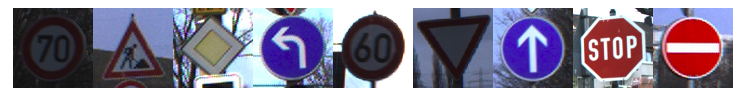
\includegraphics[width=\linewidth]{clases}
% 			\caption{Some clases}
% 			\label{fig:pipeline}
% 		\end{figure}
% 	\end{itemize}
% }


\section{Types of machine learning}

\begin{frame}
\frametitle{Machine Learning}
\framesubtitle{Types}
Depending on how machines learn: \\
\begin{itemize}
	\item \textbf{Supervised Learning.} The machine learns from labeled data.
	\item \textbf{Un-supervised Learning.} The machine tries to discover the structure of input data without labels.
	\item \textbf{Reinforcement Learning.} The machine interacts with the environment improving its actions.
\end{itemize}
\end{frame}


% Incluir 
% Generalization
\begin{frame}
\frametitle{Supervised Learning}
\begin{figure}
	\centering
	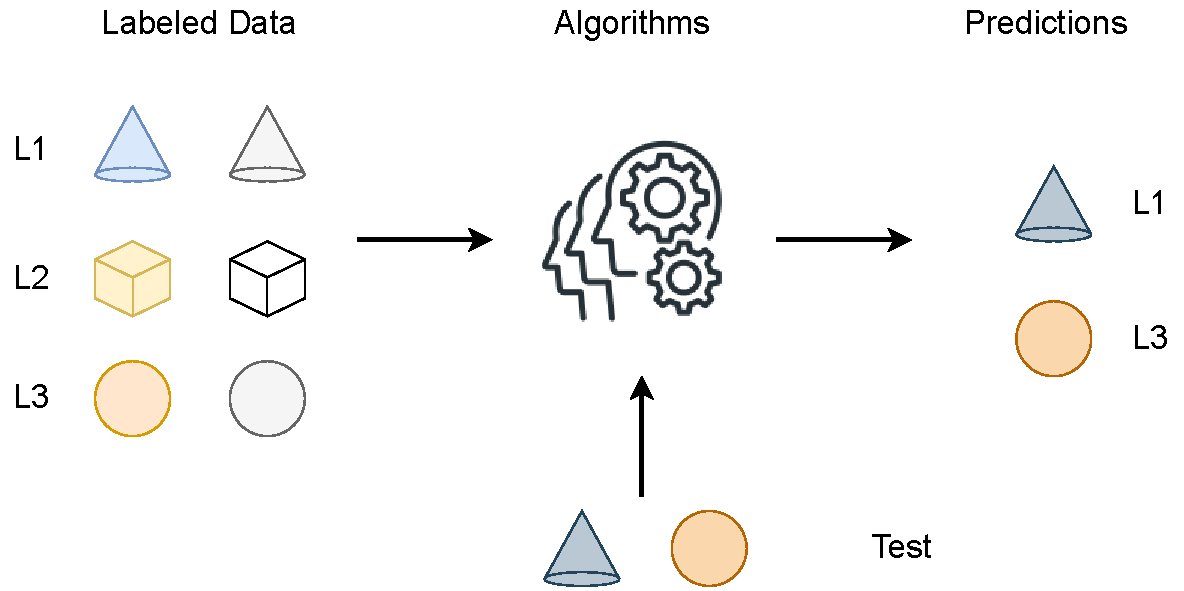
\includegraphics[height=0.6\textheight]{supervised learning.drawio.pdf}
	%\caption{}
	\label{fig:mla}
\end{figure}
\end{frame}


\begin{frame}
\frametitle{Unsupervised Learning}
\begin{figure}
	\centering
	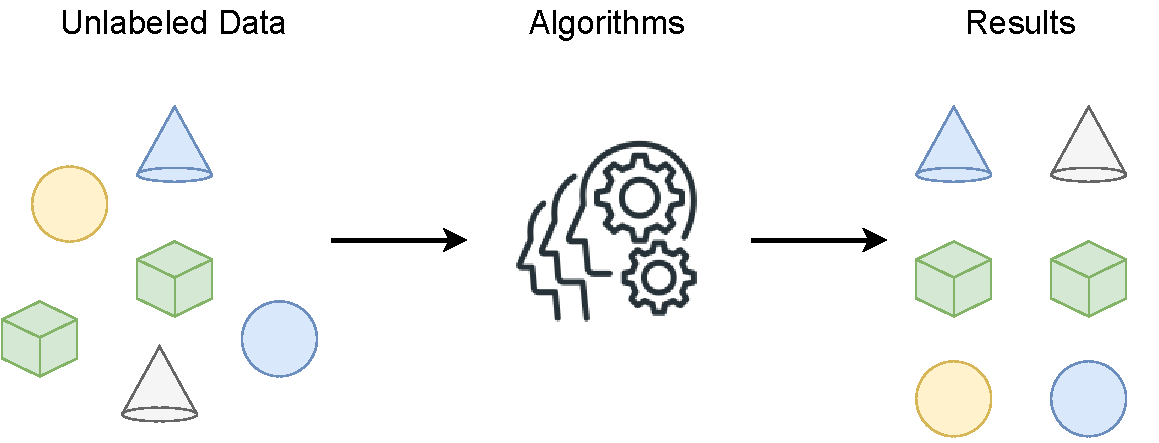
\includegraphics[height=0.5\textheight]{unsupervised learning.drawio.pdf}
	%\caption{}
	\label{fig:mla}
\end{figure}
\end{frame}

\begin{frame}
\frametitle{Reinforcement Learning}
\begin{figure}
	\centering
	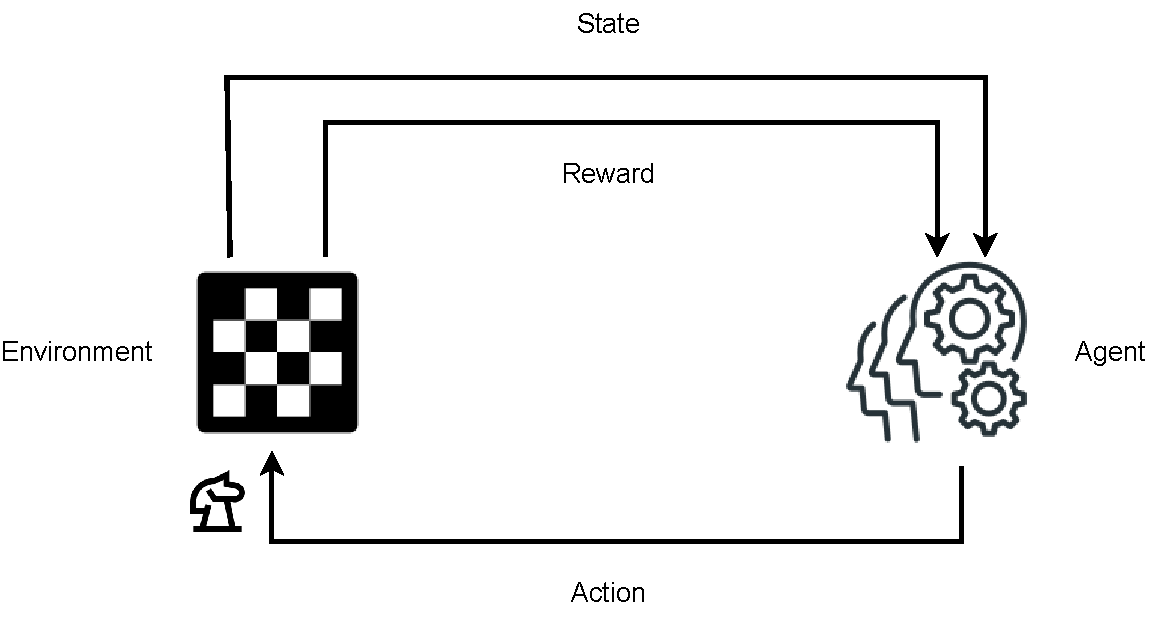
\includegraphics[height=0.7\textheight]{reinforcement.drawio.pdf}
	\label{fig:mla}
\end{figure}
\end{frame}


\begin{frame}
\frametitle{Further readings}
\begin{itemize}
	\item Sections 18.1 and 18.2, \textit{Learning from examples} chapter, Russell and Norvig, Artificial Intelligence: A modern apprach.
	\item Section 5.1 \textit{Learning Algorithms}. Goodfellow et al., Deep Learning, MIT Press.
\end{itemize}
\end{frame}



\begin{frame}
\frametitle{References}
{\footnotesize
\begin{itemize}
	\item \url{https://www.topbots.com/ai-research-generative-adversarial-network-images/}
	\item \url{https://neptune.ai/blog/dimensionality-reduction}
	\item \url{https://www.kaggle.com/c/dogs-vs-cats}
	\item \url{https://training.galaxyproject   .org/archive/2022-08-01/topics/statistics/tutorials/clustering_machinelearning/tutorial.html}
	\item Photo by charlesdeluvio on Unsplash, Photos: 
	Julie Molliver
	Shane Rounce
\end{itemize}
}
\end{frame}
%
%


\end{document}